% SPDX-FileCopyrightText: Copyright (c) 2023 Yegor Bugayenko
% SPDX-License-Identifier: MIT

\documentclass{article}
\usepackage[template,scheme=dark-mono,nominutes]{ppt-slides}
\usepackage{clicks}
\usepackage[russian]{../../lecture-notes/notes}
\usepackage{svg}
\usepackage{tikz}
  \usetikzlibrary{shadows}

\graphicspath{{../../faces/}}

\newcommand\bi[2]{#2}

\newcommand*{\thetitle}{\bi{What Can You Do For Me, Human?}{Зачем ты мне, человек?}}
\newcommand*{\thesubtitle}{}
\newcommand*{\theauthor}{\bi{Yegor Bugayenko}{Егор Бугаенко}}

\newcommand\hi[1]{\textcolor{orange}{#1}}

\pagecolor{black}

\begin{document}

\pptLeft{%
  
\includegraphics[height=3em]{sbergile-logo.png}\\
  \bi{May 23rd, 2026}{23 мая 2026}}
\pptRight{@yegor256}

\plush{
  \begin{textblock}{5}(10,0)%
    \tikz \node[minimum width=\paperwidth, minimum height=\paperheight, fill=white, inner sep=0pt] {};
  \end{textblock}%
  \begin{textblock}{8}[1,1](15,15)%
    \raggedleft%
    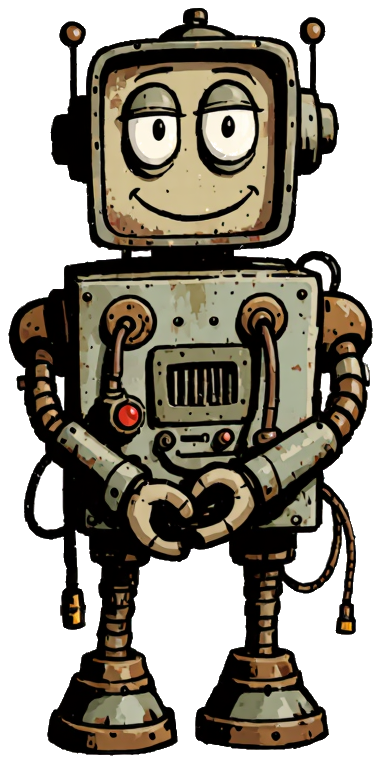
\includegraphics[width=.5\linewidth]{robot.png}
  \end{textblock}%
  \begin{textblock}{10}[0.5,0.5](6.5,7)
    \pptTitle{{\textcolor{black}{\thetitle}}}{}\par
    \textcolor{white}{\theauthor{} @ Zerocracy}\\
    \textcolor{white}{\bi{May 23rd, 2026}{23 мая 2026}}
  \end{textblock}
  \begin{textblock}{10}[0.5,0.5](6.5,12)
    
\includegraphics[height=3em]{sbergile-logo.png}
  \end{textblock}
}
\newpage

\plick{\pptBanner{\bi{I Am a Software Developer}
  {Я уже 25 лет работаю программистом}}
  \vspace*{2em}}
  \plick{\bi{Top-5 GitHub contributor in China}
    {Вхожу в топ-5 GitHub активистов (в Китае)}}
  \plick{\bi{Co-designer of EO programming language}
    {С коллегами разработал \emph{новый язык} программирования}}
  \plick{\bi{Author of seven books about coding and testing}
    {Написал семь книг о кодировании и тестировании}}
  \plush{\bi{Founder of Zerocracy, AI manager of software teams}
    {Создал Zerocracy, где ИИ управляет разработкой}}

\newcommand\pitch[6]{
  \plush{
    \pptBanner{\bi{#1}{#2}}
    \vspace*{2em}
    \enquote{\bi{#3}{#4}}\\
    \href{#5}{#6}}}

\pitch
  {Now, When AI Is Uncertain, It Asks Me}
  {Когда ИИ не знает что делать, спрашивает меня}
  {Context engineering is the delicate art and science of filling
    the context window with just the right information for the next step.}
  {Контекст-инжиниринг --- это тонкое искусство и наука наполнения
    контекстного окна именно той информацией, которая нужна для следующего шага.}
  {https://x.com/karpathy/status/1937902205765607626}
  {Andrej Karpathy, Co-Founder of OpenAI, 25 Jun 2025}

\pitch
  {Today, We Humans Are the Integrators}
  {Сегодня, мы - интеграторы}
  {Once coding speed jumps, everything around it becomes the constraint:
    clarifying requirements, reviewing changes, validating correctness and performance,
    getting to production safely.}
  {Когда скорость написания кода резко возрастает, всё остальное становится
    узким местом: уточнение требований, ревью изменений, проверка корректности
    и производительности, безопасный вывод в продакшн.}
  {https://x.com/pauldix/status/2006423514446749965}
  {Paul Dix, CTO of InfluxDB, 31 Dec 2025}

\pitch
  {Soon, AI Holds the Entire System --- We Hold the Intent}
  {Скоро: ИИ знает продукт, мы знаем замысел}
  {Humans steer. Agents execute.}
  {Люди направляют. Агенты исполняют.}
  {https://openai.com/index/harness-engineering/}
  {Ryan Lopopolo, OpenAI, 11 Feb 2026}

\pitch
  {The Flip: The Machine Will Ask Us, We Become Writers}
  {Скоро: ИИ ждет от нас прозы, ему нужны писатели}
  {Claude Code pauses for clarification more often than humans interrupt it.}
  {Claude Code останавливается за уточнениями чаще, чем люди его прерывают.}
  {https://www.anthropic.com/research/measuring-agent-autonomy}
  {Anthropic, 18 Feb 2026}

\pitch
  {Then, We Become the Senses}
  {Затем мы станем их органами чувств}
  {In a world where agents handle most cognitive processing,
    humans become the irreplaceable sensors and attestors
    of ground truth about the real world.}
  {В мире, где агенты выполняют большую часть когнитивной работы,
    люди становятся незаменимыми сенсорами и свидетелями
    истины о реальном мире.}
  {https://medium.com/\%40dmik/humans-as-sensors-why-the-agent-revolution-needs-a-new-kind-of-human-contribution-cabb57a7c2e6}
  {Dima Mikhaylov, 21 Feb 2026}

\plick{\pptBanner{\bi{Eventually, AI Will Feel Through Us}
  {В конце концов, ИИ будет чувствовать через нас}}
  \vspace*{2em}}
  \plick{\bi{AI has no feelings of its own - that's why it needs ours}
    {У ИИ нет собственных чувств - поэтому ему нужны наши}}
  \plick{\bi{What it feels like to be a person - stays ours}
    {Каково это - быть человеком - остаётся за нами}}
  \plick{\bi{Tech geeks of the past become humanitarians of the future}
    {Технари прошлого становятся гуманитариями будущего}}
  \plush{\bi{The last unexportable skill is \textbf{empathy}}
    {Последний неэкспортируемый навык - это \textbf{эмпатия}}}

\plush{\begin{pptMiddle}\ttfamily
  \bi{
    AI: "This module is messy - safe to refactor?" \\
    me: "Betty shipped it Friday - she's proud of it" \\
    AI: "OK, I'll submit a few polite improvements"}
  {ИИ: <<Этот модуль написан грязно - можно его отрефакторить?>> \\
    я: <<Бетти выкатила его в пятницу - она им гордится>> \\
    ИИ: <<Хорошо, я отправлю пару вежливых улучшений>>}\end{pptMiddle}}

\plush{\qrcode[height=12em]{https://t.me/yegor256news}}

\end{document}
